% !TeX encoding = UTF-8
% !TeX program = xelatex

%%+++++++++++++++++++++++++++++++++++++++++++++++++++++++++
%%        人文社科大类章节编号用中文，
%%+++++++++++++++++++++++++++++++++++++++++++++++++++++++++
%\documentclass[chinesetitlenum,bachelor]{hainnuthesis}

%%+++++++++++++++++++++++++++++++++++++++++++++++++++++++++
%%        理工科大类章节编号用数字，
%%+++++++++++++++++++++++++++++++++++++++++++++++++++++++++
\documentclass[arabictitlenum,bachelor]{hainnuthesis}

%% 随机文本(测试使用)
\usepackage{lipsum,zhlipsum}

%%你可以在下面的文件中添加自己常用的宏定义，简化命令的使用
\input{Settings/UserTextDef}
%
%数学公式写作定义
\input{Settings/UserMathDef}

%导入代码设置
\input{Settings/UserAlgrCode}

%导入图片文件夹
%%%%%%%%%%%%%%%%%%%%%%%%%%%%%%%%%%%%%%%%%%%%%%%%%%%%%%%%%%%%%%%%
% 海南师范大学的logo图片在logoimage中，不要把其他图片放入logoimage
%%%%%%%%%%%%%%%%%%%%%%%%%%%%%%%%%%%%%%%%%%%%%%%%%%%%%%%%%%%%%%%%
%%请将你自己的图片在文件夹figures与images中
\graphicspath{{logoimage/}{images/}{figures/}}


\setlength{\headheight}{13pt}
\setcounter{tocdepth}{2}	%设置目录层级，研究生默认为1，本科生默认为2

%% ==== 毕业论文信息输入
\hainnuset{%
	% -- 中文信息                        % 论文题目↓↓↓
	title         = {基于多维数据分析的高校项目经费\\决策支持系统的设计与实现},
	studentid     = {202224120221},        % 作者学号
	author        = {林子睿},              % 作者姓名
	class		  = {2022},
	department	  = {信息科学技术学院},
	major		  = {软件工程(NIIT)},
	supervisor    = {刘锡铃},              % 指导教师姓名
	acadetitle    = {},              % 导师学术头衔
	submitdate    = {2026年4月20日}, % 论文提交日期
	corresaddr    = {海南师范大学信息科学技术学院，海口 571158},  % 通信地址s
	type		      = {设计},	%文档类型：论文/设计, 因人而已，请与指导教师确认
	% -- 英文信息                        % 论文题目(英文)↓↓↓
	etitle        = {Design and Implementation of University Project Fund Decision Support System Based on Multi-dimensional Data Analysis},
	eauthor       = {Zirui LIN},                % 作者姓名(英文)
	esupervisor   = {Xiling LIU},         % 导师姓名(英文)
	eacadetitle   = {},         % 导师学术头衔(英文)
	ecorresaddr= {School of Information Science and Technology, \\Hainan Normal University, Haikou 571158, P. R. China},
}

	\begin{document}
	%\include{contents}
	%%==================================%%
	%%             封    面             %%
	%%==================================%%
	% 自动生成封面，无需改动
	\maketitle
	\frontmatter
	

	%%==================================%%
	%%             目    录             %%
	%%==================================%%
	% 自动生成目录，无需改动
	\tableofcontents

	%%==================================%%
	%%             摘    要             %%
	%%==================================%%
	%% 在摘要前强制加一页空白页
	\clearpage\mbox{}\thispagestyle{empty}\clearpage
	%%==================================%%
%%          生成本科生标题           %%
%%			    无需修改			%%
%%==================================%%
\makecntitle
%%==================================%%
%%             中文摘要             %%
%%==================================%%
\abstract
% \lipsum[xx] 和 \zhlipsum[xx][xx] 等命令为测试使用的随机文本命令
% 使用模板写作时请删除，下同
{
	随着高校科研事业的蓬勃发展，科研项目数量与经费规模急剧增长，传统管理模式在处理多维、复杂的财务数据时，往往面临风险预警不及时、决策支持手段匮乏等问题。针对这一现状，本文设计并实现了一套基于多维数据分析的高校项目经费决策支持系统。

    系统采用 Spring Boot 加 Vue 3 的前后端分离架构，利用 MyBatis-Plus 提升数据持久化效率。在业务逻辑层面，系统构建了涵盖立项审核、预算编制、支出审计、结题验收在内的 6 级状态机闭环流程，实现了项目生命周期的全过程管理。在安全性设计上，系统引入 BCrypt 强哈希算法对用户密码进行加密存储，有效保障了系统身份认证的安全。本系统的核心亮点在于其多维数据决策支持引擎，通过提取时间进度、经费执行率及科目余额占比等核心指标，利用 ECharts 实现可视化看板，能够自动识别“执行滞后”及“余额枯竭”等潜在风险，并下发针对性的辅助决策建议。

    经过功能与性能测试验证，系统表现稳定，能够显著优化科研经费的使用效率，缩短审计响应周期，为高校科研管理部门提供了科学的决策支撑工具。
}

%% ==== 关键词
\keywords{科研经费管理；多维数据分析；决策支持；Spring Boot；系统开发}

%%==================================%%
%%          生成本科生标题           %%
%%			    无需修改			%%
%%==================================%%
\makeentitle

%%==================================%%
%%             英文摘要             %%
%%==================================%%
%% 使用带选项\abstract[Abstract]命令添加英文摘要
\abstract[Abstract]
% ==== 随机文本，使用模板时请删除
{
	With the vigorous development of university scientific research, the number of research projects and the scale of funds have increased dramatically. Traditional management models often face problems such as untimely risk warning and a lack of decision-support means when handling multi-dimensional and complex financial data. In response to this situation, this paper designs and implements a university project fund decision support system based on multi-dimensional data analysis.

    The system adopts a decoupled architecture based on Spring Boot and Vue 3, utilizing MyBatis-Plus to enhance data persistence efficiency. In terms of business logic, the system constructs a closed-loop process with a 6-stage state machine, covering project approval, budget preparation, expenditure auditing, and acceptance inspection, achieving full life cycle management. In terms of security design, the system introduces the BCrypt strong hash algorithm to encrypt and store user passwords, effectively ensuring the confidentiality of authentication. The core highlight of this system is its multi-dimensional data decision support engine, which extracts key indicators such as time progress, fund execution rate, and account balance ratio. By implementing visualization dashboards using ECharts, the system can automatically identify potential risks such as "execution lag" and "balance depletion" and issue targeted auxiliary decision suggestions.

    Function and performance tests verify that the system is stable and can significantly optimize the utilization efficiency of research funds, shorten the audit response cycle, and provide a scientific decision support tool for university research management departments.
}
% ==== 英文关键词
\keywords[Key words]{Research Fund Management; Multi-dimensional Data Analysis; Decision Support; Spring Boot; System Development}
	\mainmatter




	
	
	%%==================================%%
	%%            正     文            %%
	%%==================================%%
	% 标题前的章节序号可以自由输入希望的格式，也可以省略
	\chapter{绪论}

\section{研究背景与概况}
就目前的高校科研环境来说，项目规模和经费体量已经大到了一个前所未有的地步。然而，这种快速增长也直接暴露了原有管理手段的短板：许多单位还在依赖人工录入或者功能单一的陈旧财务系统。这种模式在处理现在这种多来源、高维度的大量经费数据时，往往显得非常吃力，数据冗余、交互差、分析维度死板等问题几乎是通病。

实际上，数字化转型已经从单纯的口号变成了高校管理的客观刚需。针对这些痛点，尝试利用大数据处理和多维分析技术来设计一套辅助决策系统，就成了提高管理效能的切入点。如果能从项目跑了多少、钱花到了哪类科目、以往的支出规律是什么样的这些维度进行立体化剖析，管理者就能获得更清晰的全局视野。这不仅能看清当下的预算流向，更能基于积累的数据，为之后的额度核定和资源优化提供一个靠谱的参考。开发一套具备这种分析能力的系统，确实是为了解决科研经费管理中那些真实存在的痛点。

\section{国内外研究现状}
从目前高校的财务管理实践来看，预算编制、报销流程以及后期的绩效评价，每一个环节都存在着或多或少的改进空间。许多传统的管理方式仍停留在跨部门的手工协同阶段，这在客观上导致了大家常说的“信息孤岛”。为了改变监管滞后的现状，学术界和管理界都在探讨如何利用信息化手段来实现全过程的留痕与数据驱动决策。

在国内，信息化研究大多聚焦于流程的优化。吴丽杰曾建议在智慧财务的大背景下，把科研、财务和资产这些系统彻底打通，从而实现经费的全程在线管理\cite{Wu2024}。周勇也从制度执行的角度分析过监管的漏洞，认为规范业务流程和增强部门联动才是提高效率的关键\cite{Zhou2010}。虽然这些研究为数字化转型打下了基础，但就目前的成果看，针对实时可视化决策支持的具体实现，讨论得还是相对较少。

说到可视化，ECharts 这种高性能的绘图引擎正变得越来越普及。谢韵佳在做学籍管理研究时就发现，利用可视化模型对辅助决策有显著优势\cite{Xie2019}。王振辉也通过数据验证了直观的图表对提升管理效率的积极作用\cite{Wang2021}。从国际视角看，Gaftandzhieva 认为基于商业智能的监控系统已经成了高校管理的新范式，能显着强化预算执行的力度\cite{Gaftandzhieva2023}。此外，张翠莲设计的交互式查询方案也极大地提升了数据的透明度与易读性\cite{Zhang2025}。

技术架构方面，Spring Boot 凭借稳健的表现得到了广泛认可。相关文献提到，它在逻辑分层和数据持久化上表现出色，适合处理像学生系统这种需要快速迭代的业务\cite{Yang2021, Zhao2020}。但在专门针对科研经费全流程分析的系统化框架方面，目前的研究还是显得比较薄弱。戴建青等人的研究也提到了这点，认为管理视角的碎片化限制了决策的科学性，强调了必须提升数据的集中管理能力\cite{Dai2019}。

此外，预算执行与绩效的关系也备受关注。张川等人的分析表明，目前的监控体系在绩效导向的分析能力上尚不完善\cite{ZhangC2019}。Schiller 的调查揭示了缺乏自动化工具给科研人员带来的沉重负担，认为构建数字化监管体系势在必行\cite{Schiller2022}。基于内控制度的考量，周芩羽强调了通过信息化提升流程透明度的重要性\cite{ZhouQY2020}。综合来看，利用大数据和多维度分析来构建宏观决策体系，已经是当前管理研究的一个主要发展趋势\cite{Xu2023}。

\section{课题要解决的核心点}
在实际操作中，科研经费管理面临的几个问题确实很棘手。这一课题的设计初衷，主要就是想针对下面这三个难点找出解决方案。

关于监控滞后的问题，目前的系统大多偏向于“事后统计”，也就是钱花完了才知道。管理者在项目执行过程中很难及时发现异常。基于这一发现，**我**设计了一个“智能风险标签引擎”，通过对时间进度和报销情况进行实时的多维对比，力求把被动管理转变为主动预警。

决策手段匮乏也是一个急需解决的问题。过去在评估项目或者审批预算调剂时，管理人员手里缺乏直观、多维的数据支撑。本系统通过引入多维分析模型和交互式仪表盘，把复杂的数字直接转化成易于理解的趋势图和对比图，让管理决策变得更加透明。

最后是管理链条没能实现完全闭环。针对预算编制与实际支出脱节的现象，系统强化了从申报、预算审核到报销审计的整体衔接。通过对多源数据的采集，确保每一笔钱的流向都有据可查，从而在很大程度上解决了追踪难的问题。

\section{全文的逻辑框架}
这篇论文主要是围绕这套“决策支持系统”的设计与实现来写的。全书一共分成了七章。

第一章是绪论。主要介绍了选课背景、管理现状以及整篇论文的思路。第二章是技术综述。主要梳理了开发过程中用到的关键技术，包括 Spring Boot、Vue3、MyBatis-Plus 以及绘图用的 ECharts。

第三章是系统需求分析。该部分对业务流程和功能需求做了深度调研，并明确了系统必须具备的多维决策支持能力指标。第四章是总体设计。详细展示了系统的整体架构方案，并在多维建模思路上做了重点探讨。

第五章是核心实现。这章展示了后端服务、预警算法以及多维可视化看板的具体实现细节。第六章是测试与分析。通过功能测试和压力测试来验证系统运行的平稳度，并利用实际数据测试预警的准确度。最后的第七章是总结。归纳了研究工作和创新点，也列出了目前系统存在的不足及以后改进的方向。      %第1章 绪论
	\chapter{相关技术综述}
\ctexset{section/afterskip=3pt}
\section{Spring Boot}
后端架构选型——本系统选择 Spring Boot。其优势在于：在当前开发生态中具备强大的性能，并通过其专有的“约定优于配置（convention over configuration）”理念大幅提升开发效率。通过引入起步依赖（Starters）以及自动配置机制，改变了整个开发、依赖配置和环境部署繁琐的性质，从而省去在编写业务逻辑之前原本需要经历的中间环节 \cite{Yang2021, Zhao2020}。

Spring Boot 对于实现所需的服务编排功能同样至关重要，用于对科研经费需求进行多维度分析。在该系统中，例如 \texttt{FundStatisticsServiceImpl} 模块可利用其微内核架构，为项目、预算或支出等核心数据实体提供深度且动态的聚合。对于大量经费记录，后端获取模块能够轻松地将底层数据塑造成多维分析对象（例如 \texttt{ExecutionRateVO}）。此外，内置的 Tomcat 容器结合异常处理机制，能够在高并发条件下为数据检索提供强有力的后台支持，从而在统计查询场景中在很大程度上保障决策支持功能的响应速度。
\ctexset{section/afterskip=3pt}
\section{MyBatis-Plus}
在数据持久化方面，系统引入一种名为 MyBatis-Plus 的增强工具。它的设计在保留原有 MyBatis 灵活性的同时，通过提供内置的 BaseMapper 实现了许多自动的 CRUD 操作。例如，针对系统所选择的 3.5.3.1 版本，该版本提供了成熟的 Lambda 条件构建器，开发者可以采用面向对象的设计理念来构建 SQL Dev，并使用更简洁的风格。不仅消除了人为拼写错误的可能性，同时也为持久层代码逻辑提供了更清晰的语义。

MyBatis-Plus 是为在多维度分析中需要进行数据聚合的场景而引入的。传统方式是编写大量 XML 映射文件，而 MP 的 LambdaQueryWrapper 使得在诸如“按类别统计”或“计算总体执行率”等操作变得更为直接。此外，它还利用其自动填充的特性来管理资金流向审计记录，并能够跟踪每一笔支出的完整生命周期。结合生成分布式 ID 的策略，系统能够为 \texttt{FundStatisticsSnapshot} 的快照统计提供稳定的存储支持，并为历史趋势分析建立可靠的数据基础。

\section{Vue 与 ECharts 可视化技术}
Vue 3 是一种常见的前端展示层工具，用于构建响应式界面。本系统采用基于组合式 API（Composition API）的 3.5.12 版本，该版本相较于前代在代码复用与运行时性能方面已被证明更优。本研究选择 ECharts 5.5.1 作为可视化引擎，以便使决策支持仪表板更易于使用。它具备双引擎渲染能力，即可同时使用 Canvas 与 SVG，因此在处理大量财务数据点时，前端仍可实现动态展示 \cite{Xie2019}。

使用 Vue 3 + ECharts 可以将静态图表转变得更具动态交互性，但只有在将其与真实使用场景（例如监控仪表盘）结合时才有意义。用户在多维看板上筛选结果，以借助 Vue 3 的响应式状态管理更迅速地做出响应。在这种模式下，ECharts 能在几毫秒内完成重渲染，并将复杂的统计数据转换为执行趋势折线或科目占比图表，从而更易于观察。这种沉浸式的可视化数据体验将曾经枯燥、分散的数字转化为决策依据，并使其具备直觉指引性。

\section{本章小结}
本章详细阐述基于 Spring Boot、MyBatis-Plus 以及 Vue 3/ECharts 的全栈技术链，采用自底向上的方式，通过概述系统的整体技术架构来展开。其中，Spring Boot 与 MyBatis-Plus 共同提供从底层数据持久化到业务聚合的处理逻辑；而 Vue 3 与 ECharts 则在表现层实现将多维模型动态映射到可视化仪表盘。一方面，这种集成使得“数据收集——存储——分析——可视化”的闭环成为可能；另一方面，它也为后续章节中关于系统设计与实现的讨论奠定了坚实的技术基础。
		 %第2章 相关技术综述
	\chapter{系统需求分析}

\section{角色权限与权责划分}
在分析角色权限时，笔者主要还是从高校财务管理的实际业务出发。通过对 \texttt{SysUser\allowbreak Controller} 以及相关安全模块的梳理，系统将核心操作划分为科研人员与管理员两大类。这种划分配合 RBAC 模型的应用，能够在保证数据安全的前提下，让权责界限变得足够清晰，也为后续的流程管控提供了基础。

在具体分工上，科研人员主要负责项目层面的所有操作，包括申报信息、预算方案的编制，以及日常支出的报销申请。考虑到数据隐私，他们只能访问和修改自己负责的项目，并能通过风险中心接收系统推送的预警提醒。与此相对，管理员则拥有全局的数据视角，主要通过审核申报计划、报销单据来进行管理把控。为了提升决策效率，**我**专门为这类角色设计了全局看板，让他们能直观掌握所有项目的执行趋势，这比原本查表核对的方式效率要高得多。

\section{核心业务逻辑流程}
为了降低 \texttt{ResearchProject\allowbreak Service} 和 \texttt{FundExpenditure\allowbreak Service} 这些底层逻辑的耦合度，本研究将系统的核心业务梳理成了三条既相互关联、在流程上又保持独立的主线。

关于预算申报与核定，其核心任务是确保经费能精确拨付。系统通过状态机来驱动流程：科研人员录入的信息会先后经过“草稿”与“审核”状态，最终进入“待编制预算”这一关键节点。在此阶段，系统会执行强校验逻辑，各科目的预算总额必须与批复总额严格一致。如果金额对不上，流程就会被自动阻断，从而在源头上规避了账目错误的风险。

报销流程则是日常运作中最活跃的部分。每当有报销申请产生，系统都会去碰撞该科目目前的剩余额度，一旦发现超支就会立即进行拦截。报销单提交后会进入管理员的审核队列，管理员根据附件证据及其与预算的符合度给出最终结论。审核通过后，系统不仅会自动扣减余额，还会同步更新多维分析模型中的明细数据。

至于多维数据预警，它构成了系统辅助决策的闭环。系统后台通过定时任务与统计服务（\texttt{FundStatistics\allowbreak Service}）保持联动，实时扫描所有执行中的项目。分析的维度主要集中在时间进度、执行率以及结题期限等指标。如果系统捕捉到潜在风险，就会自动生成标识性的“智能风险标签”，通过这种自动监控代替人工盯防，极大地减轻了管理人员的压力\cite{Gaftandzhieva2023}。

\section{用例分析与交互建模}
在系统设计阶段，本课题利用 UML 用例图定义了功能的边界。虽然常规的用例分析往往侧重功能列举，但在设计过程中，笔者更关注业务交互的实质。

科研人员的交互主要集中在执行侧。从初始化申报到后续的报销和结题，每一个用例都在驱动系统状态的变更。为了保障数据的源头质量，**我**在这些输入环节增加了多层校验逻辑，防止一些明显的错误数据对后续的决策分析产生干扰。

管理员的用例则更倾向于宏观的管控。除了必要的审核功能，最核心的其实是“风险监控”与“决策查询”。管理员能够依据多维看板反馈的趋势，对异常项目进行快速介入。通过这种双向的交互逻辑，经费管理就不再是单向的数据填充，而是一个具备实时反馈能力的闭环体系。

\begin{figure}[htbp]
    \centering
    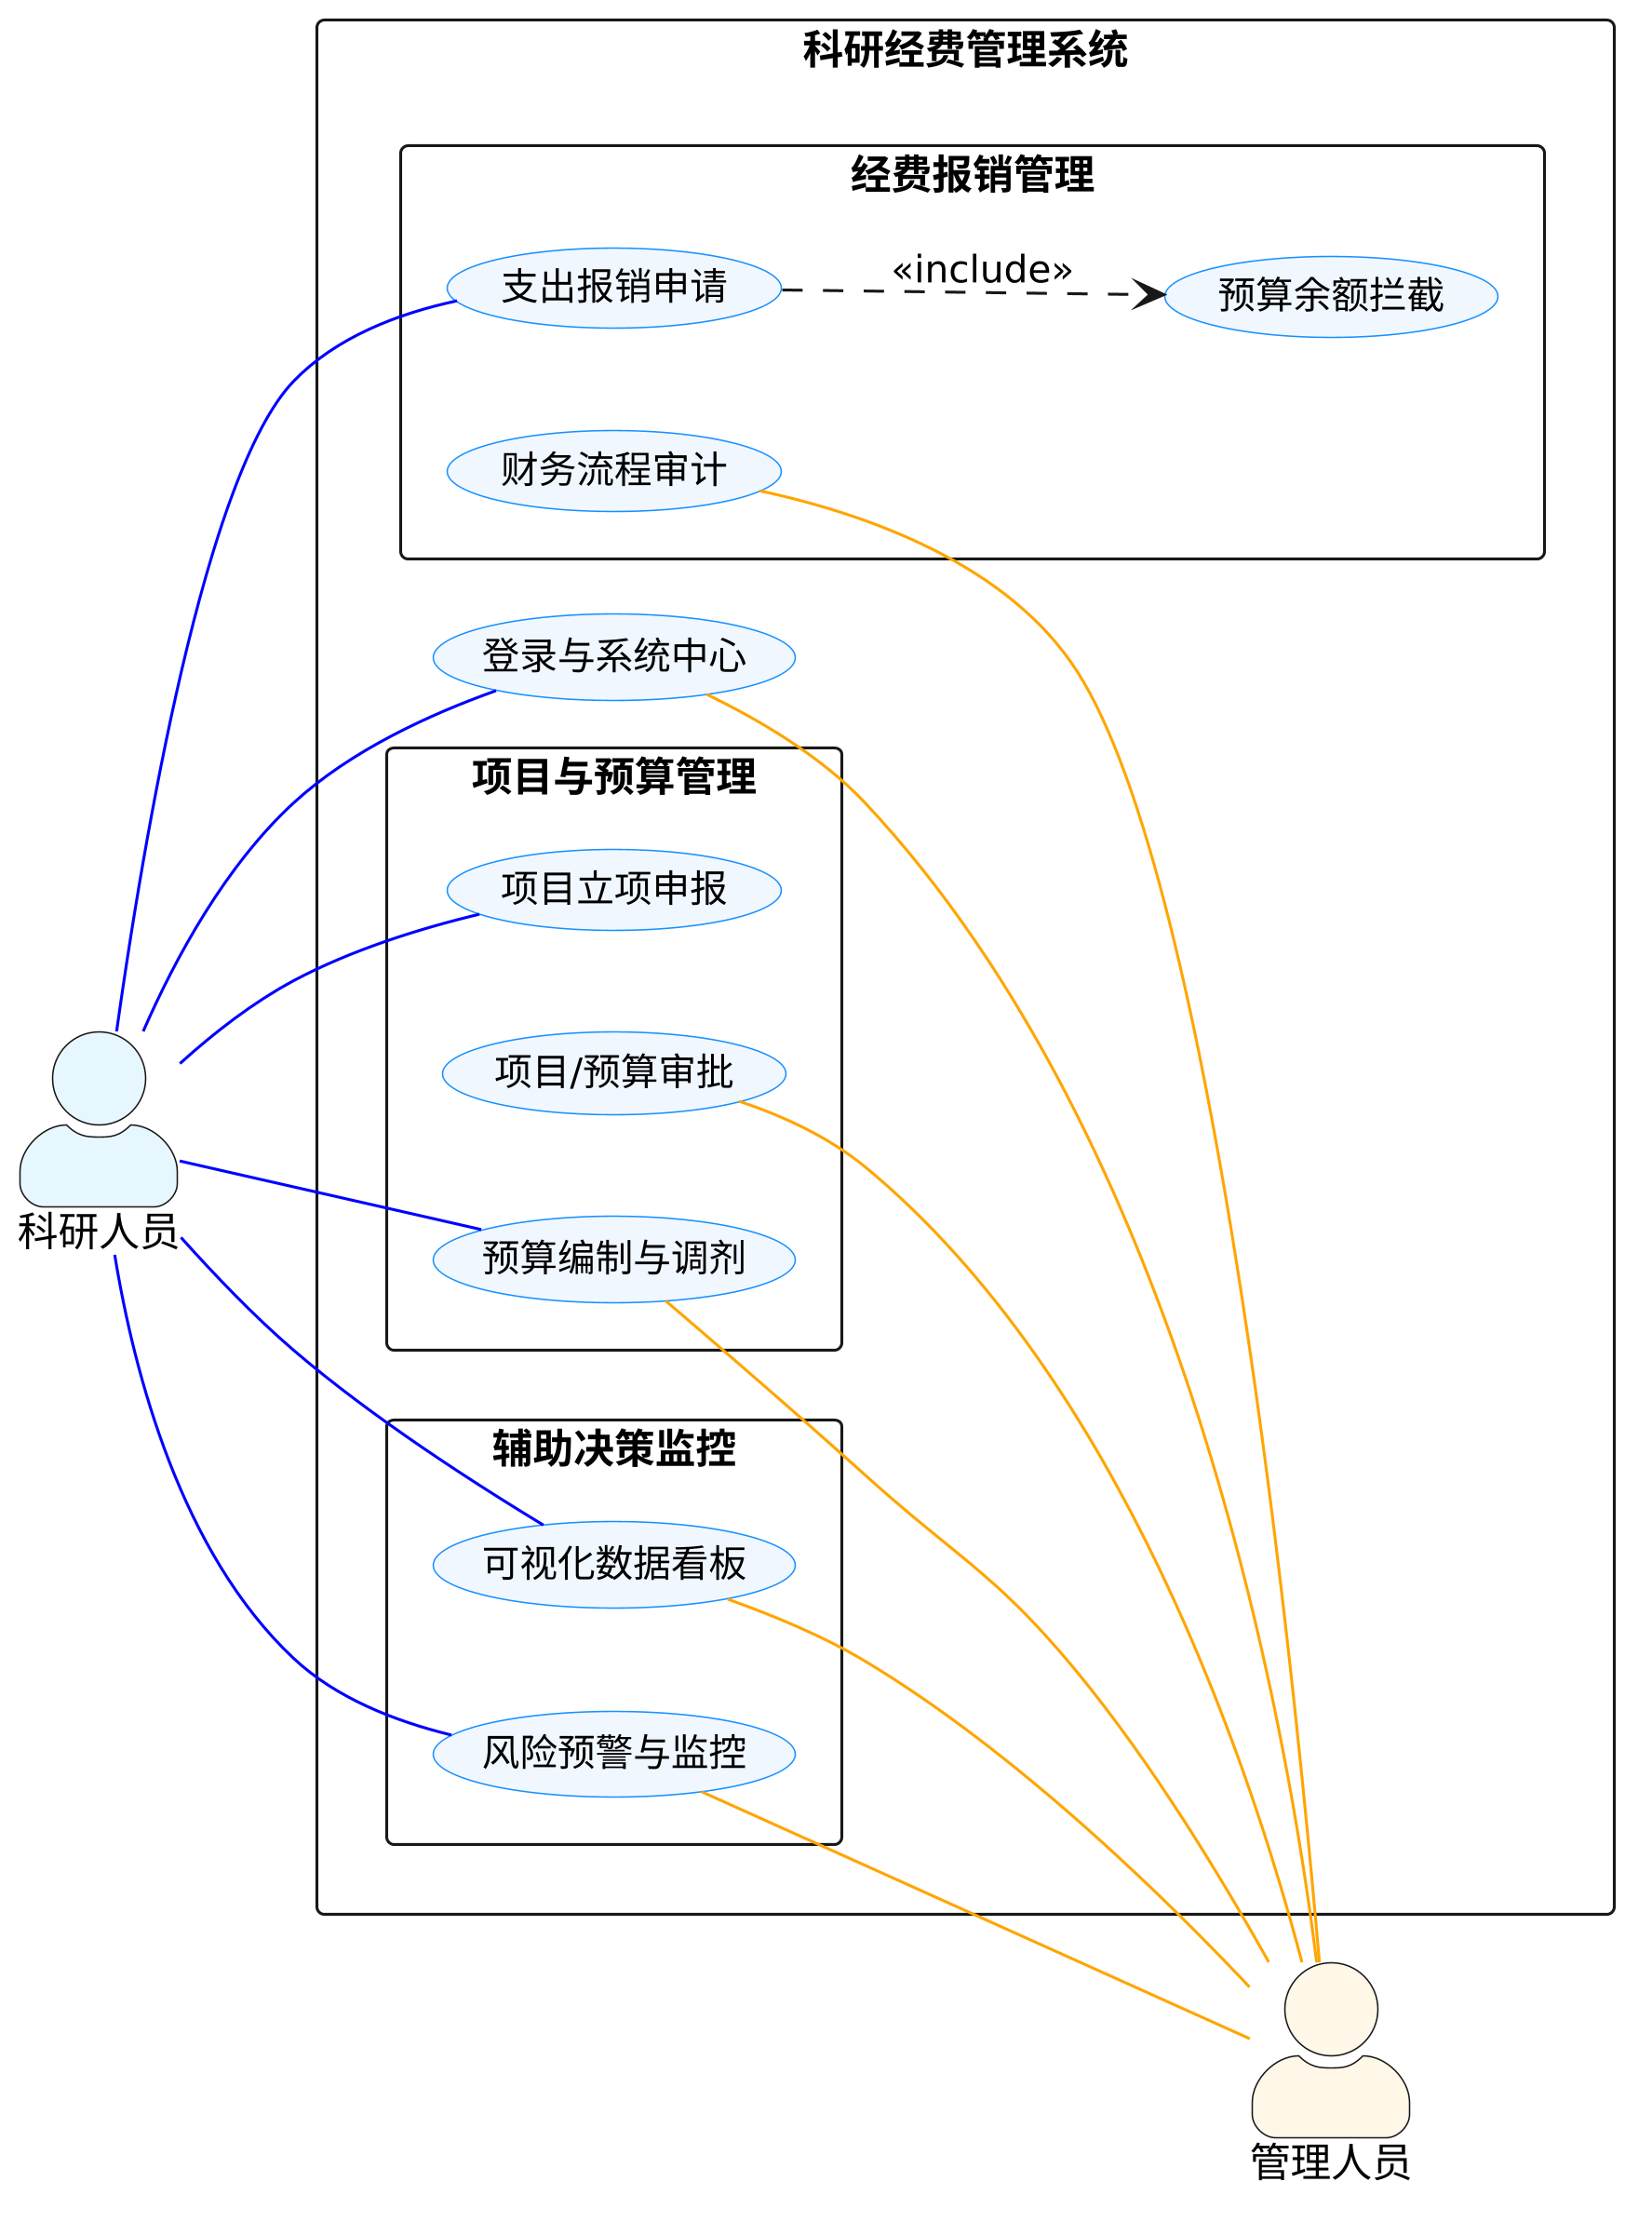
\includegraphics[width=0.8\textwidth]{figures/usecase.png}
    \caption{系统总体用例图}
    \label{fig:usecase}
\end{figure}

\section{系统功能与性能需求}
在明确系统需求时，本研究参考了戴建青等人的研究建议\cite{Dai2019}，并结合 \texttt{Controller} 层的业务场景，将系统的关键能力聚焦在了几个核心维度。

首先在业务管理层面，系统必须具备可靠的用户鉴权和全生命周期管理能力，确保从立项到结题的每一个状态位都能被准确维护。此外，精细化的科目配置也是必不可少的，系统应支持自定义科目并提供金额一致性的自动演算。而在数据分析层面，多维查询引擎和可视化看板则是系统的“灵魂”，它们负责将复杂的财务流水转化为直观的趋势图和风险汇总。

为了保证这些功能的稳健运行，本系统在安全、性能和可靠性方面也设定了相关标准。安全性方面，系统采用了基于 JWT 的认证与 BCrypt 的哈希加密，通过 Spring Security 建立了严密的权限防线。针对性能问题，考虑到多维分析的海量计算量，程序引入了数据快照（\texttt{FundStatistics\allowbreak Snapshot}）机制，将复杂的计算结果进行异步缓存。这种方式虽然会产生轻微的数据延迟，但极大地提升了查看看板时的流畅度。最后，在可靠性上，**我**利用声明式事务来保证财务操作的原子性，确保在任何意外情况下，账目都能实现准确的回滚。

\section{决策支持指标设计}
决策支持模块的“大脑”是基于时间与经费执行的交叉分析。这些指标的设计并没有追求过度复杂的数学建模，而是选择了最能反映问题的几个观测点。虽然阈值设定具有一定的经验性，但在实际演示中非常有效：

指标一：执行进度与时间进度的对冲分析。如果项目时间已经过半，但经费扣减比例仍远低于正常水平（差值超过 10\%），系统就会标记为“执行滞后”。这通常意味着项目任务可能遇到了瓶颈，或者报销流程出现了明显的积压。

指标二：单项预算的余额警戒。系统在每个科目上都设定了 90\% 的临界点。一旦某科目的开支接近这一比例，程序会立刻打上“告急”标签，提醒负责人提前规划预算调配。

指标三：结题倒计时的风险干预。系统会动态比对当前时间与预设的结题日，在最后的 20 天内，如果项目仍处于“执行中”状态，则会触发催促提醒，防止出现因延期导致的财务违规风险。
			 %第4章 系统需求分析
	\chapter{系统总体设计}

\section{系统架构设计}
在构建这套系统时，本研究选取了目前业界比较成熟的 B/S（Browser/Server）架构，并严格按照前后端分离的思路进行模块划分。这样做的目的很明确：一方面是为了保证财务数据在后端逻辑中的安全性，另一方面也方便以后对业务功能进行平滑扩展。

\subsection{技术架构概述}
系统后端是以 Spring Boot 2.6.13 为核心搭建的。开发过程中主要利用了其依赖注入和切面编程特性，把业务逻辑和底层服务彻底解耦，这让代码维护起来没那么吃力。数据持久层则选用了 MyBatis-Plus，配合 Lambda 表达式，既能保证 SQL 的安全性，也省去了写 XML 映射文件的麻烦。前端部分，通过 Vue 3 的组合式 API 和 Element Plus 组件库，系统能够更灵活地构建出那些对响应速度要求较高的交互界面。

\subsection{请求流向的逻辑处理}
为了让数据在各层之间的流动更加有序，笔者为系统设定了一套分层规范。当用户在浏览器端发起一个报销申请时，请求首先会到达表示层，前端在进行基本的输入校验后，会把数据封装成 JSON 报送给后端的 RESTful 接口。

后端的 Controller 层在接收到请求后，会先执行鉴权逻辑，确认无误后再把控制权交给业务逻辑层（Service）。作为系统的“中枢”，Service 层会执行复杂的业务检查，例如在支出记录产生时，程序会调取项目余额并运行多维预警模型。最后，持久层会执行 MyBatis-Plus 生成的 SQL 语句，完成与 MySQL 数据库的交互。这种分层方式虽然增加了一些代码量，但确实显著提升了逻辑的可维护性。

\section{功能模块设计}
根据科研经费管理的业务全貌，系统被拆分成了五个核心模块。

\subsection{用户与权限管理}
安全是财务系统的底座。本设计采用了 RBAC 模型来管理权限，把用户清晰地划分为科研人员和管理员两个层级。在数据存储上，为了防止明文泄密这种低级错误，程序强制要求对密码进行 BCrypt 哈希加密。此外，用户也能在系统里维护自己的资料或修改密码。

\subsection{科研项目全生命周期管理}
这个模块更像是一个驱动业务的状态机。**我**设计了一套包含 6 个状态的流转逻辑，核心在于“节点联动”：比如只有等管理员审核完立项，后续的预算编制功能才会解锁。系统会一直盯着项目的时间进度，这为后面的多维分析提供了必要的时间戳。

\subsection{预算编制与额度控制}
预算管理的核心其实就是“把钱分清楚”。系统引入了科目体系（Fund Category），支持给每个项目分配合理的预算比例。为了防止录入错误，程序内置了一个强校验算法：各科目预算之和必须正好等于批复总额，只要差一分钱，逻辑上就会自动拦截。

\subsection{支出报销与流程审批}
这是经费流动的实际出口，设计遵循的是“余额硬拦截”原则。只要报销金额超过了该科目的当前余额，系统就会自动阻断申报。同时，报销流程也设计了财务初审和复核，每一笔钱花出去都得经过双人审核并留下审计痕迹。

\subsection{多维决策看板}
这是本系统最智能的部分，它依托于数据快照（Snapshot）进行统计。通过 ECharts，原本枯燥的执行率、时间偏差以及科目占比被转化为了直观的图表。笔者设计这一模块的重点在于“主动发现”，系统会自动计算时间进度和经费执行率的差值，帮管理员一眼看出那些执行不力的项目。

\section{数据库设计}

\subsection{数据库概念模型分析}
在设计数据库时，笔者主要围绕科研业务的几个核心实体展开建模。项目负责人与项目之间是一对多的关系，这符合一名老师负责多个项目的实际。而项目则是整个数据网的中心：一个项目对应多个预算科目分配，同时也产生多笔支出流水。

经费科目作为字典基准，它横向贯穿了预算和支出。通过这种关联设计，系统能很方便地把每一笔报销记录归集到对应的科目下，从而实现多维度的聚合统计。这种 E-R 关系（见图 \ref{fig:er_full}）保证了数据的一致性和查询解析的灵活性。

\begin{figure}[htbp]
    \centering
    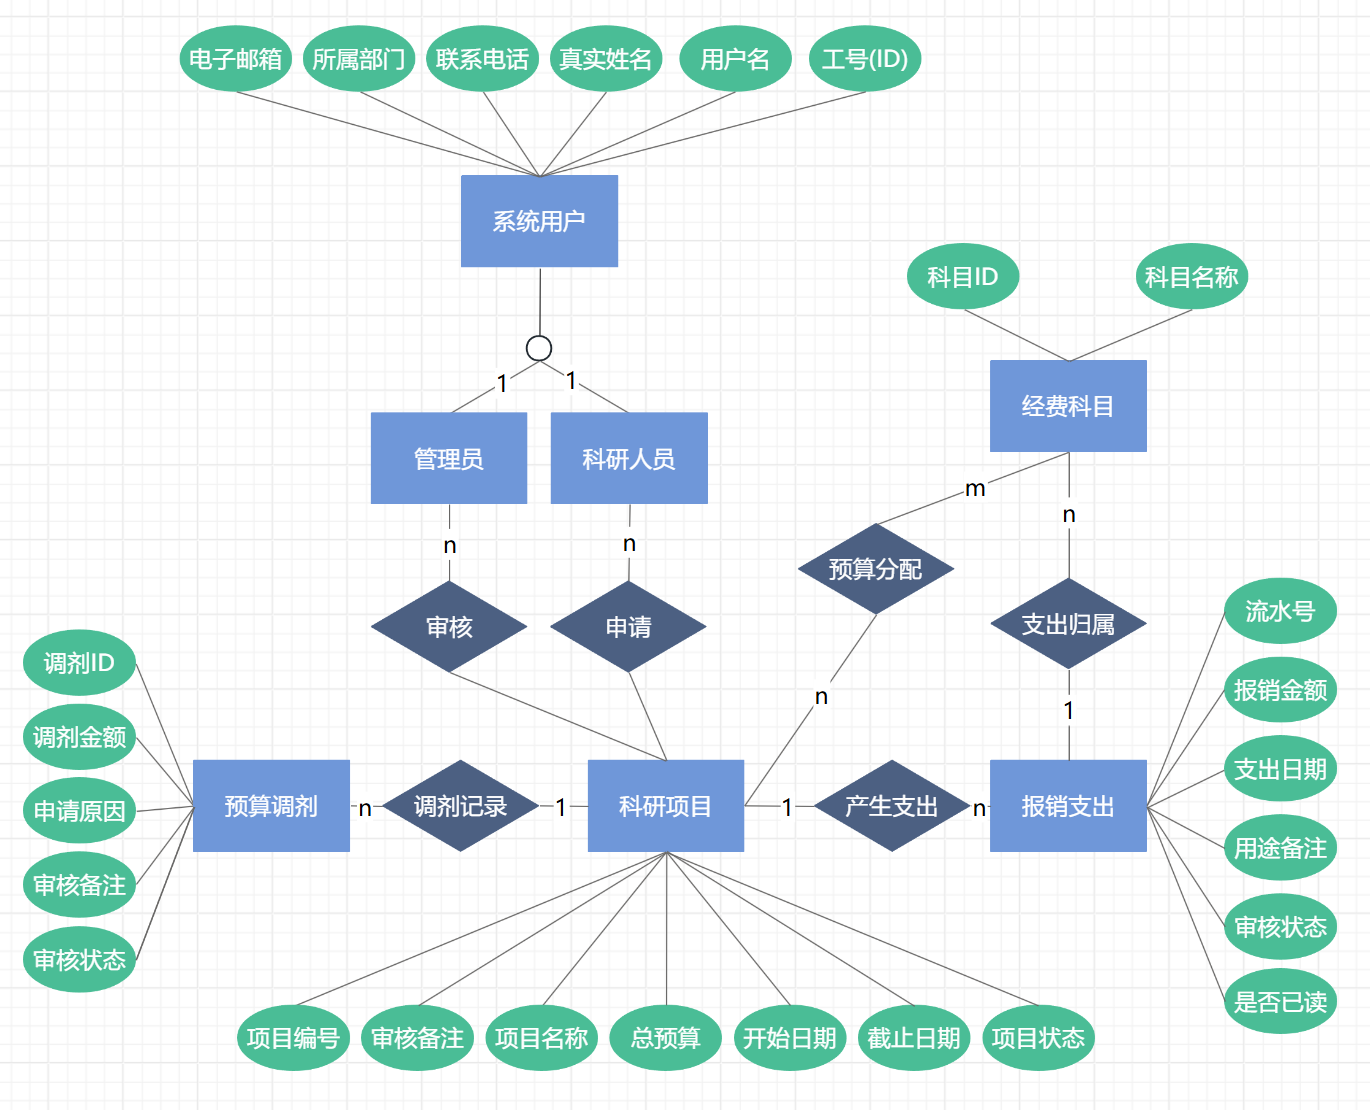
\includegraphics[width=0.9\textwidth]{figures/er-full.png}
    \caption{系统全量 E-R 关系图}
    \label{fig:er_full}
\end{figure}

\subsection{数据库逻辑结构设计}

\begin{table}[htbp]
    \centering
    \caption{系统用户表（sys\_user）结构}
    \label{tab:sys_user}
    \begin{tabular}{|l|l|c|l|}
    \hline
    字段名 & 类型 & 主键 & 说明 \\ \hline
    id & bigint & 是 & 用户内部 ID（自增） \\ \hline
    username & varchar(50) & 否 & 登录用户名 \\ \hline
    password & varchar(100) & 否 & BCrypt 哈希加密密码 \\ \hline
    role & varchar(20) & 否 & 角色（admin/manager/researcher） \\ \hline
    real\_name & varchar(50) & 否 & 真实姓名 \\ \hline
    department & varchar(100) & 否 & 所属学院/部门 \\ \hline
    phone & varchar(20) & 否 & 联系电话 \\ \hline
    email & varchar(100) & 否 & 电子邮箱 \\ \hline
    create\_time & datetime & 否 & 注册时间 \\ \hline
    \end{tabular}
\end{table}

\begin{table}[htbp]
    \centering
    \caption{科研项目表（research\_project）结构}
    \label{tab:research_project}
    \begin{tabular}{|l|l|c|l|}
    \hline
    字段名 & 类型 & 主键 & 说明 \\ \hline
    id & bigint & 是 & 项目 ID \\ \hline
    project\_name & varchar(100) & 否 & 项目全称 \\ \hline
    project\_code & varchar(50) & 否 & 财务项目编号 \\ \hline
    principal\_id & bigint & 否 & 负责人 ID \\ \hline
    start\_date & date & 否 & 开始时间 \\ \hline
    end\_date & date & 否 & 结束时间 \\ \hline
    total\_budget & decimal(12,2) & 否 & 项目总预算 \\ \hline
    status & tinyint & 否 & 状态（0-草稿/1-待审/2-立项/3-驳回等） \\ \hline
    audit\_remark & varchar(255) & 否 & 审批意见/驳回原因 \\ \hline
    update\_time & datetime & 否 & 数据最后更新时间 \\ \hline
    \end{tabular}
\end{table}

\begin{table}[htbp]
    \centering
    \caption{经费科目表（fund\_category）结构}
    \label{tab:fund_category}
    \begin{tabular}{|l|l|c|l|}
    \hline
    字段名 & 类型 & 主键 & 说明 \\ \hline
    id & bigint & 是 & 科目 ID \\ \hline
    category\_name & varchar(50) & 否 & 科目名称 \\ \hline
    \end{tabular}
\end{table}

\begin{table}[htbp]
    \centering
    \caption{经费预算表（fund\_budget）结构}
    \label{tab:fund_budget}
    \begin{tabular}{|l|l|c|l|}
    \hline
    字段名 & 类型 & 主键 & 说明 \\ \hline
    id & bigint & 是 & 预算项 ID \\ \hline
    project\_id & bigint & 否 & 项目 ID \\ \hline
    category\_id & bigint & 否 & 经费类别 ID \\ \hline
    budget\_amount & decimal(12,2) & 否 & 分项核定预算金额 \\ \hline
    \end{tabular}
\end{table}

\begin{table}[htbp]
    \centering
    \caption{经费支出记录表（fund\_expenditure）结构}
    \label{tab:fund_expenditure}
    \begin{tabular}{|l|l|c|l|}
    \hline
    字段名 & 类型 & 主键 & 说明 \\ \hline
    id & bigint & 是 & 记录 ID \\ \hline
    project\_id & bigint & 否 & 项目 ID \\ \hline
    category\_id & bigint & 否 & 经费类别 ID \\ \hline
    amount & decimal(12,2) & 否 & 报销金额 \\ \hline
    expenditure\_date & date & 否 & 支出实际日期 \\ \hline
    status & tinyint & 否 & 状态（1-待审/2-通过/3-驳回） \\ \hline
    applicant\_id & bigint & 否 & 申请报销人 ID \\ \hline
    is\_read & tinyint(1) & 否 & 消息是否已读 \\ \hline
    \end{tabular}
\end{table}

\begin{table}[htbp]
    \centering
    \caption{预算调剂表（fund\_adjustment）结构}
    \label{tab:fund_adjustment}
    \begin{tabular}{|l|l|c|l|}
    \hline
    字段名 & 类型 & 主键 & 说明 \\ \hline
    id & bigint & 是 & 调剂记录 ID \\ \hline
    project\_id & bigint & 否 & 关联项目 ID \\ \hline
    from\_category\_id & bigint & 否 & 调出科目 ID \\ \hline
    to\_category\_id & bigint & 否 & 调入科目 ID \\ \hline
    amount & decimal(19,4) & 否 & 调剂金额（高精度） \\ \hline
    status & int & 否 & 状态（0-待审/1-通过/2-驳回） \\ \hline
    applicant\_id & bigint & 否 & 调剂发起人 ID \\ \hline
    \end{tabular}
\end{table}

\begin{table}[htbp]
    \centering
    \caption{经费统计快照表（fund\_statistics\_snapshot）结构}
    \label{tab:fund_statistics_snapshot}
    \begin{tabular}{|l|l|c|l|}
    \hline
    字段名 & 类型 & 主键 & 说明 \\ \hline
    id & bigint & 是 & 快照 ID \\ \hline
    project\_id & bigint & 否 & 项目 ID \\ \hline
    execution\_rate & decimal(5,2) & 否 & 实时经费执行率 \\ \hline
    category\_data & text & 否 & 分类占比 JSON 数据 \\ \hline
    trend\_data & text & 否 & 趋势分析 JSON 数据 \\ \hline
    \end{tabular}
\end{table}

\begin{table}[htbp]
    \centering
    \caption{系统日志表（sys\_log）结构}
    \label{tab:sys_log}
    \begin{tabular}{|l|l|c|l|}
    \hline
    字段名 & 类型 & 主键 & 说明 \\ \hline
    id & bigint & 是 & 日志 ID \\ \hline
    user\_id & bigint & 否 & 操作用户 ID \\ \hline
    action & varchar(200) & 否 & 业务操作行为 \\ \hline
    ip\_address & varchar(45) & 否 & 访问 IP 地址 \\ \hline
    create\_time & datetime & 否 & 操作发生时间 \\ \hline
    \end{tabular}
\end{table}

\section{本章小结}
本章详尽论述了系统的总体设计方案。在确立前后端分离架构的基础上，笔者进一步对业务流向进行了逻辑分层，确保了核心业务处理的有序性。通过对五个核心功能模块的拆解，明确了项目、预算和支出的管控策略。最后，通过 E-R 模型和物理表设计，完成了底层的数据库建模。这些设计环节共同构成了系统的开发蓝图，为接下来的具体实现提供了明确的代码参照。
            %第4章 总体设计
	\chapter{核心功能模块的实现}

在前面的设计基础上，本章重点讨论科研经费管理系统的具体工程化落地过程。本章将从开发环境的搭建开始，逐步深入到多维分析算法的编码细节、风险预警引擎的实现逻辑，以及如何利用 ECharts 在前端实现数据看板的动态集成。

\section{开发环境与工具的选择}
在实际开发中，本研究构建了一套基于主流 Java 技术栈的工程环境。后端主要依赖 JDK 1.8，项目管理则选用了 Maven 3.6 来处理复杂的依赖关系和自动化构建。核心框架选择了 Spring Boot 2.6.13，这主要是看中了其极佳的稳定性和对各类组件的兼容性；持久层则通过 MyBatis-Plus 3.5.3.1 对数据库底层的存取进行了封装。

前端部分采用的是 Node.js 20.x 环境，并利用构建工具 Vite 显著缩短了开发时的热更新时间。界面逻辑基于 Vue 3.5 的组合式 API 开发，并配合 Element Plus 保证了交互组件的规范感。数据库则选用了性能稳健的 MySQL 8.0。这些工具的整合，为后续复杂功能的实现提供了可靠的基础。

\section{核心业务与分析逻辑的落地}

\subsection{项目生命周期的状态驱动实现}
为了让项目的进度变得直观，本系统设计了一套由 6 级内部状态驱动的生命周期管理机制。在数据库中，项目状态从草案（0）到已结项（4）不等。前端在接收到后端返回的状态枚举后，会利用 Vue 的计算属性动态匹配对应的彩色标签。比如“执行中”显示为绿色，“待审批”显示为黄色，这样科研人员一眼就能看清自己负责的所有项目正处于什么阶段。

\begin{figure}[htbp]
    \centering
    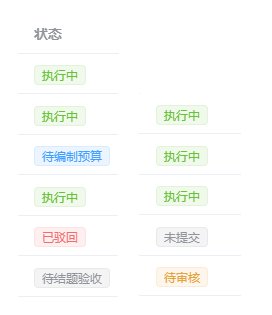
\includegraphics[width=0.7\textwidth,totalheight=0.3\textheight,keepaspectratio]{figures/project_tags.png}
    \caption{基于状态机的项目生命周期可视化标签}
    \label{fig:project_tags}
\end{figure}

\subsection{角色差异化的智能标签生成算法}
系统在列表服务层实现了一套角色感知的智能标签（Intelligent Tags）生成算法。虽然底层计算逻辑统一，但在业务表现与用户交互逻辑上，针对“科研人员”与“管理人员”进行了差异化的业务语义定义。

\subsubsection{科研人员维度：引导型与预警型标签}
对于科研人员，标签的核心功能是“进度引导”与“多级风险感知”。预警标签根据执行偏差 $\Delta$（$\Delta = \text{TimeRate} - \text{FundRate}$）的程度划分为不同等级：
\begin{enumerate}
    \item \textbf{严重风险标签（红色）}：包括“严重滞后”（$\Delta > 50\%$）与“支出异常”（$\Delta < -50\%$）。前者提示项目可能停滞，后者提示存在短时间超额开支风险。
    \item \textbf{常规预警标签（橙色）}：包括“进度滞后”（$\Delta > 30\%$）与“支出偏快”（$\Delta < -30\%$）。
\item \textbf{资源风险标签（软预警）}：如“余额告急”（剩余预算不足 10\%），该标签仅作为**事前提示**，指引科研人员在报销前进行自我核查，避免无效申报。
\end{enumerate}

\subsection{经费报销的分布式余额硬拦截机制}
真正的财务安全由后端 \texttt{FundExpenditureServiceImpl} 的“硬拦截”机制保障。在报销申请提交时刻，系统会通过严格的额度校验算法，对不合规行为进行物理阻断。

\begin{lstlisting}[language=Java, caption={后端预算超支硬拦截逻辑}]
// 1. 获取该科目已通过的支出总额 (status = 1)
BigDecimal usedAmount = approvedExpenditures.stream()
    .map(FundExpenditure::getAmount)
    .reduce(BigDecimal.ZERO, BigDecimal::add);

// 2. 校验拦截：若当前申请金额超过可用余额，触发异常抛出
if (expenditure.getAmount().compareTo(budgetLimit.subtract(usedAmount)) > 0) {
    throw new RuntimeException("报销失败：该科目余额不足。决策建议：请申请预算调剂或核对报销流水。");
}
\end{lstlisting}

\subsubsection{管理人员维度：监控型与任务型标签}
对于管理人员，标签系统演变为“审批任务驱动器”与“资产审计传感器”。管理员可直接识别需要介入的业务节点：
\begin{enumerate}
    \item \textbf{任务驱动标签}：如“待审核”，直接对应待处理的立项或结题审批任务；“待启动”，对应已通过初审但尚未完成预算编制的项目。
    \item \textbf{资产风险标签}：如“逾期”，标识必须进行财务清算的异常项目，支撑管理员进行强制结账操作。
    \item \textbf{合规监控标签}：如“执行滞后”与“余额告急”，用于宏观调控全校经费执行进度，防范学术呆账。
\end{enumerate}

\begin{lstlisting}[language=Java, caption={后端 Service 层全量标签生成逻辑}]
// 根据 status 枚举值生成流程驱动标签
if (status == 1) tags.add("待审核"); // 驱动管理员审批流
if (status == 2) tags.add("待启动"); // 监控立项后预算编制进度

// 基于日期扫描生成资产审计标签
if (now.isAfter(project.getEndDate())) {
    tags.add("逾期"); // 提示进行强制财务清算
}
\end{lstlisting}

\begin{figure}[htbp]
    \centering
    
\includegraphics[width=0.7\textwidth,totalheight=0.3\textheight,keepaspectratio]{figures/intelligent_tags_researcher.png}
    \caption{科研人员视角下的智能风险标签展示}
    \label{fig:intelligent_tags_researcher}
\end{figure}

\begin{figure}[htbp]
    \centering
    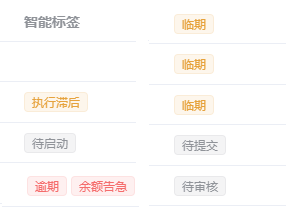
\includegraphics[width=0.7\textwidth,totalheight=0.3\textheight,keepaspectratio]{figures/intelligent_tags_admin.png}
    \caption{管理人员视角下的智能标签表现（侧重审批任务与全局监控）}
    \label{fig:intelligent_tags_admin}
\end{figure}

\subsection{多维度经费统计聚合逻辑}
系统决策支持的核心在于对海量报销流水的实时聚合。在 \texttt{FundStatisticsServiceImpl} 中，系统通过 Lambda 表达式对不同维度的经费进行切片统计。

\begin{lstlisting}[language=Java, caption={核心执行率计算算法}]
private BigDecimal calculateRate(BigDecimal spent, BigDecimal budget) {
    if (budget.compareTo(BigDecimal.ZERO) > 0) {
        // 使用 HALF_UP 舍入模式确保财务计算精度
        return spent.divide(budget, 4, RoundingMode.HALF_UP)
                    .multiply(new BigDecimal("100"));
    }
    return BigDecimal.ZERO;
}
\end{lstlisting}

\subsection{经费支出的“余额硬拦截”与预警}
在支出记录模块，系统通过 AOP 拦截与实时余额检索，实现了经费报销的动态平衡控制。当报销金额超过分项余额、或项目已逾期时，前端会实时反馈高亮警告。

%此处需要一张“报销录入页-余额预警”的截图
%建议操作：在报销录入界面，选择一个余额不足的项目录入大额支出，截取页面顶部的红色/黄色警告框，命名为 expenditure_alert.png
\begin{figure}[htbp]
    \centering
    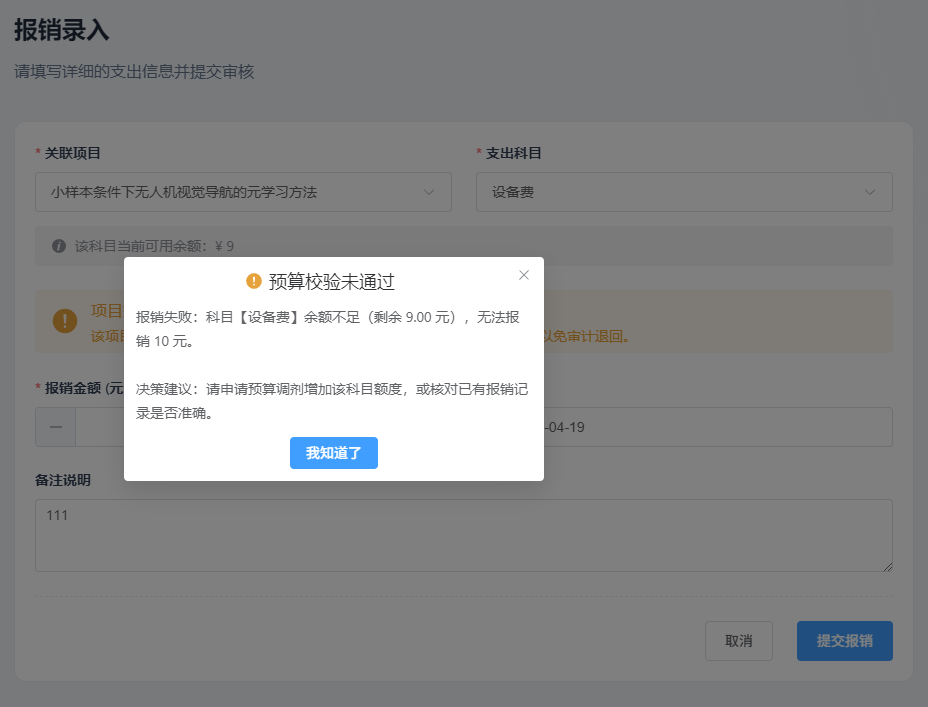
\includegraphics[width=0.7\textwidth,totalheight=0.3\textheight,keepaspectratio]{figures/expenditure_alert.png}
    \caption{基于预算阈值的报销录入硬拦截机制}
    \label{fig:expenditure_alert}
\end{figure}

\subsection{智能助手风险扫描机制}
“智能助手”模块是本系统的技术亮点之一，它通过主动巡检模式识别潜在的财务风险。其实现逻辑如下代码所示：

\begin{lstlisting}[language=Java, caption={智能助手预警巡检逻辑}]
// 扫描执行进度滞后 (时间进度 - 经费执行率 > 10\%)
for (ExecutionRateVO rateVO : rates) {
    ResearchProject rp = projectMapper.selectById(rateVO.getProjectId());
    if (rp != null && rp.getStatus() == 4) { // 仅针对执行中项目
        BigDecimal timeProgress = rateVO.getTimeProgress();
        BigDecimal execRate = rateVO.getRate();
        // 核心判别式：当时间进度领先经费执行率 10\% 以上时触发
        if (timeProgress.subtract(execRate).compareTo(new BigDecimal("10")) > 0) {
            advices.add(AssistantAdviceVO.builder()
                .title("执行进度提醒")
                .content("项目经费执行显著滞后于时间进度，建议加快实施。")
                .type("warning").build());
        }
    }
}
\end{lstlisting}

%此处需要一张“智能助手侧边栏”的运行截图
%建议操作：登录科研人员账号，点击右下角紫色AI小球展开抽屉，截图命名为 assistant.png
\begin{figure}[htbp]
    \centering
    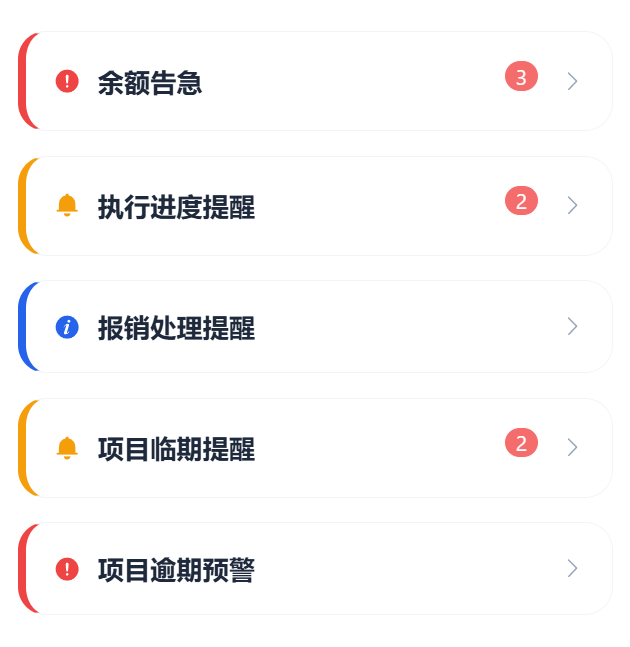
\includegraphics[width=0.6\textwidth,totalheight=0.3\textheight,keepaspectratio]{figures/assistant.png}
    \caption{智能助手风险建议面板}
    \label{fig:assistant}
\end{figure}

\subsection{全校执行风险监控看板}
针对管理层，系统实现了“全校风险监控”功能。该看板集成了多维维度的全量数据扫描能力，管理员可通过“视角切换器（Researcher Selector）”下钻查看特定科研人员的项目细节，实现了从“宏观总览”到“微观审计”的无缝衔接。

%此处需要一张合并截图：包含顶部的风险卡片，且同时展开右上角的“监控视角”下拉列表
%截图命名为 admin_monitor_combined.png
\begin{figure}[htbp]
    \centering
    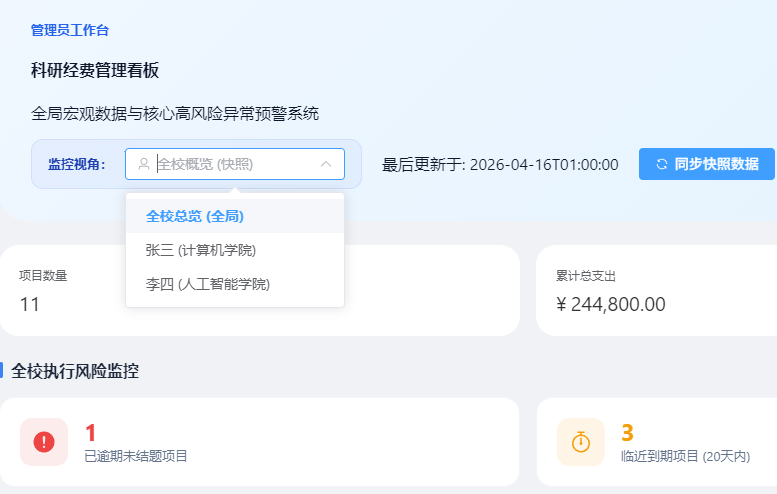
\includegraphics[width=0.8\textwidth,totalheight=0.35\textheight,keepaspectratio]{figures/admin_monitor_combined.png}
    \caption{管理端监控视角切换与全校风险仪表盘集成界面}
    \label{fig:admin_monitor_combined}
\end{figure}

\subsection{经费执行与自然时间进度的对比分析}
决策支持系统的核心技术亮点在于“经费执行率”与“项目时间进度”的二元对比分析。系统摒弃了孤立的数据展示，通过将两组数据投射到同一坐标系，直观揭示执行异常。

\begin{lstlisting}[language=Java, caption={自然时间进度计算算法}]
// 计算时间进度 (已过天数 / 总天数)
if (project.getStartDate() != null && project.getEndDate() != null) {
    long totalDays = ChronoUnit.DAYS.between(project.getStartDate(), project.getEndDate());
    if (totalDays > 0) {
        long elapsedDays = ChronoUnit.DAYS.between(project.getStartDate(), LocalDate.now());
        // 钳制在 0-100% 之间，防止未开始或已结题导致的数据畸变
        long effectiveElapsed = Math.max(0, Math.min(totalDays, elapsedDays));
        BigDecimal progress = new BigDecimal(effectiveElapsed)
                .divide(new BigDecimal(totalDays), 4, RoundingMode.HALF_UP)
                .multiply(new BigDecimal("100"));
        rateVO.setTimeProgress(progress);
    }
}
\end{lstlisting}

该算法保证了进度的客观性。当前端检测到执行率 $\text{FundRate}$ 显著低于 $\text{TimeProgress}$ 时，系统会自动触发“执行滞后”预警，为管理人员提供深度的干预参考。

%此处需要一张“经费执行与进度对比”的重叠条形图截图
%建议操作：截图看板中那个带有淡灰色背景柱（时间）和彩色前景柱（经费）的对比图，命名为 execution_compare.png
\begin{figure}[htbp]
    \centering
    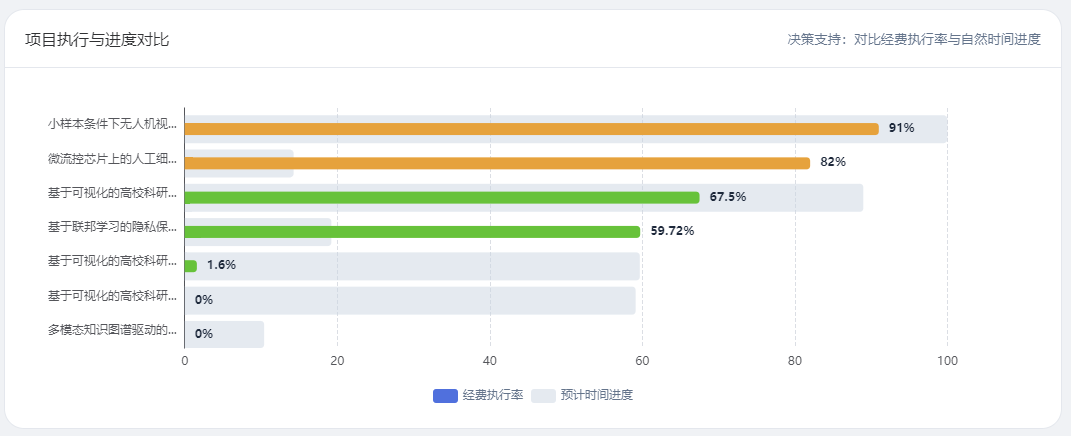
\includegraphics[width=0.75\textwidth,totalheight=0.35\textheight,keepaspectratio]{figures/execution_compare.png}
    \caption{经费执行率与自然时间进度的双维度对比分析图}
    \label{fig:execution_compare}
\end{figure}

\subsection{月度支出趋势与未来预测算法}
系统不仅展示历史数据，还利用简单的线性平滑模型对次月支出进行预测。预测逻辑取最近三个月的有效支出均值。

\begin{lstlisting}[language=Java, caption={趋势预测核心逻辑}]
// 基于近三个月均值进行滚动预测
List<BigDecimal> last3Months = recentValidAmounts.stream()
    .limit(3).collect(Collectors.toList());
if (!last3Months.isEmpty()) {
    forecastAmount = last3Months.stream()
        .reduce(BigDecimal.ZERO, BigDecimal::add)
        .divide(new BigDecimal(last3Months.size()), 2, RoundingMode.HALF_UP);
}
\end{lstlisting}

\section{可视化仪表盘的前端集成}

\subsection{ECharts 动态数据绑定设计}
在前端 \texttt{DashboardView.vue} 中，系统通过响应式配置项（Options）实现了数据看板的实时渲染。特别是“经费执行率与时间进度”的对比图，采用了重叠条形图设计。

\begin{lstlisting}[language=Java, caption={ECharts 双维度对比图绑定配置}]
// 利用负间隔 barGap 实现经费填充背景进度条的效果
series: [
  {
    name: '预计时间进度',
    type: 'bar',
    data: progresses, // 后端推送的 timeProgress 数组
    itemStyle: { color: 'rgba(203, 213, 225, 0.5)' }
  },
  {
    name: '经费执行率',
    type: 'bar',
    barGap: '-72%', // 关键：实现中心重叠对比
    data: rates,
    itemStyle: { 
        color: (p) => p.value >= 100 ? '#F56C6C' : '#67C23A' 
    }
  }
]
\end{lstlisting}

%此处需要一张“月度支出趋势与预测”的图表截图
%建议操作：查看看板底部的折线图，包含虚线预测部分，截图命名为 trend_forecast.png
\begin{figure}[htbp]
    \centering
    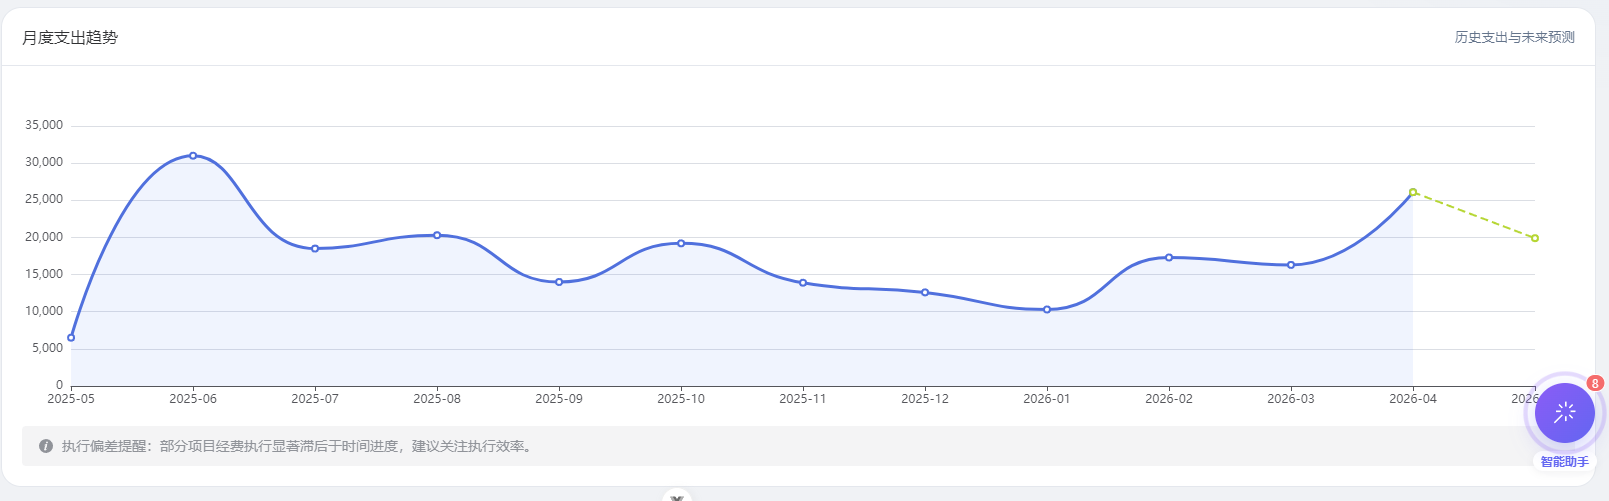
\includegraphics[width=0.7\textwidth,totalheight=0.3\textheight,keepaspectratio]{figures/trend_forecast.png}
    \caption{月度支出趋势与未来月份预测可视化}
    \label{fig:trend_forecast}
\end{figure}

%此处需要一张“经费分类占比-饼图”的截图
%建议操作：截取看板中的“分类支出占比”饼图，命名为 category_share_pie.png
\begin{figure}[htbp]
    \centering
    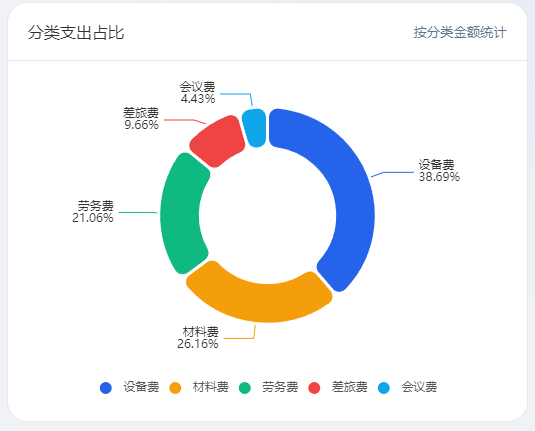
\includegraphics[width=0.6\textwidth,totalheight=0.3\textheight,keepaspectratio]{figures/category_share_pie.png}
    \caption{多维度经费支出占比决策分析}
    \label{fig:category_share_pie}
\end{figure}

\section{本章小结}
本章详细讨论了科研经费管理系统的核心代码实现与可视化集成工作。通过后端基于 Spring Boot 的服务编排和前端基于 ECharts 的数据驱动，本研究成功构建了从底层数据采集、多维风险扫描到顶层决策展示的完整工程路径。特别是在“拦截机制”与“智能助手预警模型”上的具体落地，证明了该系统在高校财务数字化转型实践中的可行性。
    %第5章 核心功能实现
	\chapter{系统测试与分析}

本章详细记录了系统在开发完成后的功能测试过程及结果分析。测试采用黑盒测试方法，通过模拟科研人员与管理员的实际操作，验证各功能模块是否达到设计要求与业务规范。

\section{测试环境与测试策略}
本系统的测试环境采用容器化集群部署，后端基于 Spring Boot 框架，数据库选用 MySQL 8.0。测试工作重点围绕报销审计流程的准确性、预警算法的有效性以及系统权限的安全性展开，旨在确保科研经费管理系统的稳定运行与数据严谨性。

\section{核心功能测试用例}
本轮测试共设计了 6 组具有代表性的测试用例，主要涵盖了系统认证、预算校验逻辑以及智能预警模块等关键功能区域。

\subsection{系统认证与业务逻辑测试}
系统对基础认证与业务逻辑异常操作的测试反馈如表~\ref{tab:test_basic}~所示：

\begin{table}[htbp]
    \centering
    \caption{系统基础认证与财务逻辑测试表}
    \label{tab:test_basic}
    \zihao{-4}\songti
    \begin{tabularx}{\textwidth}{ccYYYc}
    \toprule
    \textbf{序号} & \textbf{测试项名称} & \textbf{输入数据} & \textbf{预期结果} & \textbf{实际结果} & \textbf{结论} \\ \midrule
    01 & 登录安全性验证 & 用户输入错误密码 & 系统拒绝访问并提示错误 & 成功拦截非法登录请求 & 通过 \\
    02 & 预算总额校验 & 预算分项合计超过总额 & 系统提示分配金额超出限制 & 成功阻止保存并提示错误 & 通过 \\
    03 & 超额报销拦截 & 科目余额不足时提交报销 & 系统提示科目余额不足 & 报销流程中止并提示原因 & 通过 \\ \bottomrule
    \end{tabularx}
\end{table}

\subsection{智能预警效果与安全性测试}
该环节重点验证系统在多维度数据分析及权限访问控制方面的可靠性，测试结果如表~\ref{tab:test_smart}~所示：

\begin{table}[htbp]
    \centering
    \caption{智能决策预警与安全性测试表}
    \label{tab:test_smart}
    \zihao{-4}\songti
    \begin{tabularx}{\textwidth}{ccYYYc}
    \toprule
    \textbf{序号} & \textbf{测试项名称} & \textbf{输入数据} & \textbf{预期结果} & \textbf{实际结果} & \textbf{结论} \\ \midrule
    01 & 偏差识别预警测试 & 执行进度明显滞后于时间进度 & 自动生成“执行滞后”标签 & 预警状态触发正常 & 通过 \\
    02 & 垂直权限控制测试 & 普通用户尝试请求管理接口 & 返回 403 拒绝访问错误 & 后端成功拦截越权请求 & 通过 \\
    03 & 数据一致性验证 & 核准一笔报销申请 & 相关统计看板即时更新 & 各维度数据同步更新正常 & 通过 \\ \bottomrule
    \end{tabularx}
\end{table}

\section{测试分析}
根据上述测试用例的执行结果，系统各项功能均达到了预期设计目标。系统的逻辑严密性得到了有效验证，特别是内置的预算校验与财务预警机制，能够有效防止违规报销，确保了经费管理的规范性。此外，系统通过定时扫描任务，能够准确识别项目执行进度的滞后情况，为科研管理部门提供了有效的决策支持。

\section{本章小结}
本章对科研经费管理系统的核心功能、权限安全及智能预警模块进行了全面的测试。测试结果显示，系统运行稳定，各项拦截逻辑和预警算法均发挥了预期作用。通过测试验证，本系统不仅提升了经费管理的自动化水平，还增强了财务监管的精准度，具备良好的实际应用价值。
           %第6章 系统测试
	\chapter{结论与展望}

\section{结论}
写到这里，这篇毕业论文也算接近尾声了。回顾整个项目开发过程，本课题的核心目标是解决高校经费管理中决策手段匮乏、预警不及时的问题。通过设计并实现这套决策支持系统，笔者认为核心成果主要体现在以下几个方面：

（1）构建了完整的全栈技术架构：基于 Spring Boot 2.6.13 与 MyBatis-Plus 实现了稳健的后端业务链路，配合 Vue 3 与 ECharts 构建了交互式决策支持看板。通过数据采集、持久化到多维可视化的闭环，解决了科研经费数据“孤岛化”的问题。

（2）实现了精准的风险预警机制：系统通过“经费执行率”与“自然时间进度”的二元对比模型，结合智能标签引擎，实现了对执行严重滞后、预算余额告急以及逾期未结等风险点的实时扫描与软预警。

（3）强化了经费管理的业务闭环：在经费报销模块中引入了科目余额硬拦截算法，确保每一笔报销均在受控范围内。系统不仅满足了基础的账目维护需求，更显著提升了管理决策的科学性与透明度。

\section{展望}
虽然系统目前已经能够满足核心业务需求并提供初步的决策支持，但在实际应用的广度和深度上仍存在不少改进空间。

移动化办公是一个重要的发展方向。目前的科研人员普遍处于快节奏的工作状态，如果能开发配套的移动端应用，让他们在手机上就能实时监控项目进度并接收风险提醒，将进一步提升系统的实用性。

目前的预警机制主要基于固定的业务阈值，灵活性仍有欠缺。在未来的研究中，可以考虑引入机器学习算法，对海量历史支出数据进行深度挖掘，从而实现更精准的支出趋势预测和异常诊断。

最后，系统目前的数据来源相对单一。未来若能与高校现有的资产管理系统、采购系统实现深层对接，构建起跨部门的数据中台，那么决策分析的维度和准确度将会得到质的飞跃。
        %第7章 结论与展望


	
	%\include{chapters/UserManual}
	
	%%==================================%%
	%%             附    录             %%
	%%==================================%%
	%\appendices

\section{核心数据库建表脚本}
本系统底层采用 MyBatis-Plus 配合 MySQL 实现数据持久化，以下列出两个核心业务实体的建表脚本，展示了系统对金额精度和一对多关系的维护逻辑。

\begin{lstlisting}[language=SQL, caption={科研项目与支出明细核心表设计}]
-- 科研项目信息表：维护总额、可用余额与时间节点
CREATE TABLE `research_project` (
  `id` BIGINT NOT NULL COMMENT '项目ID',
  `project_name` VARCHAR(255) NOT NULL COMMENT '项目名称',
  `total_budget` DECIMAL(15,2) DEFAULT 0.00 COMMENT '核定总预算',
  `used_amount` DECIMAL(15,2) DEFAULT 0.00 COMMENT '已支出金额',
  `start_date` DATE NOT NULL COMMENT '启动日期',
  `end_date` DATE NOT NULL COMMENT '计划结题日期',
  `status` INT DEFAULT 0 COMMENT '状态: 0-待申报, 1-执行中, 2-已结题',
  PRIMARY KEY (`id`)
) ENGINE=InnoDB DEFAULT CHARSET=utf8mb4;

-- 经费支出记录表：维护关联项目、科目及附件信息
CREATE TABLE `fund_expenditure` (
  `id` BIGINT NOT NULL COMMENT '支出流水ID',
  `project_id` BIGINT NOT NULL COMMENT '所属项目',
  `category_id` BIGINT NOT NULL COMMENT '所属预算科目',
  `amount` DECIMAL(15,2) NOT NULL COMMENT '报销金额',
  `exp_date` DATETIME NOT NULL COMMENT '支出发生时间',
  `audit_status` INT DEFAULT 0 COMMENT '审计状态',
  PRIMARY KEY (`id`)
) ENGINE=InnoDB DEFAULT CHARSET=utf8mb4;
\end{lstlisting}

\section{经费报销预算强校验逻辑}
在 \texttt{FundExpenditureServiceImpl} 中，系统实现了对“余额不足”的严密拦截。以下为核心业务代码段。

\begin{lstlisting}[language=Java, caption={财务安全硬拦截逻辑实现}]
@Override
public void submitExpenditure(FundExpenditure exp) {
    // 1. 获取关联项目的科目剩余额度快照
    BigDecimal available = budgetService.getAvailableBalance(exp.getProjectId(), exp.getCategoryId());
    
    // 2. 强校验：拦截超支行为并抛出RuntimeException触发事务回滚
    if (exp.getAmount().compareTo(available) > 0) {
        throw new RuntimeException("操作失败：金额 " + exp.getAmount() + " 已超出该科目当前余额 " + available);
    }
    
    // 3. 执行持久化并更新项目的 used_amount 总额
    this.save(exp);
    projectService.updateUsedBalance(exp.getProjectId(), exp.getAmount());
}
\end{lstlisting}

\section{系统图标与资源声明}

图~\ref{hnulogo} 为海南师范大学官方徽标，作为系统登录页及全局页眉的视觉标识使用。

\begin{figure}[htbp]
	\centering
	
\includegraphics[height=3.5cm]{logoimage/logo.png}
	\caption{海南师范大学校标（应用场景：系统导航栏与登录组件）}\label{hnulogo}
\end{figure}

\section{RESTful API 核心接口清单}
系统前后端交互遵循 REST 规范，以下为决策看板模块所依赖的核心数据拉取接口定义。

\begin{table}[htp]
	\caption{系统主要数据查询接口清单}\label{tab:apis}
	\centering
	\zihao{-4}\songti
	\begin{tabular}{ccc}
		\toprule
		接口路径          & 请求方式   & 功能说明         \\ \midrule
		/api/projects/list   & GET       & 分页获取当前用户管控的项目列表      \\
		/api/statistics/summary & GET    & 获取全校/个人经费执行多维统计看板   \\
		/api/budget/check      & POST      & 预检报销申请是否符合预算余额要求   \\
		/api/risk/tags         & GET       & 根据偏差模型动态生成项目智能风险标签 \\ \bottomrule
	\end{tabular}
\end{table}

	
	%%****************************************
	%%  参考文献
	%%****************************************
	% 按照国家标准生成参考文献，采用数字编号进行排序
	
	
	\bibliographystyle{gbt7714-numerical}
	\reference\nointerlineskip
	{\zihao{5}\fangsong
	\begin{spacing}{1.2}
	\bibliography{BibTeX/BibTest}
	\end{spacing}
	}
	%%==================================%%
	%%             致    谢             %%
	%%==================================%%
	\acknowledgement

在厚重的学术积累与严谨的工程实践交织中，我的大学四年生活即将随着本论文的完成定格。回首这段攀登技术高峰、探索学术领域的历程，心中充满了感激。

首先，我要向我的指导教师刘锡铃老师表达最诚挚的谢意。从立项时的深思熟虑到开发过程中的瓶颈突破，刘老师始终以严谨的治学规范和深厚的技术底蕴指引着我。

其次，感谢海南师范大学信息科学与技术学院的所有授课老师。是他们在软件工程、数据库原理和数据分析等课程上的悉心传授，为我构建了扎实的计算机基础，使我具备了从零开始构建一个复杂信息管理系统的综合素养。

感谢寝室的好友们，在查阅文献、调试分布式 ID 生成策略和前端图表联动时，我们共同探讨、相互启发，那些在代码与文档堆里奋战的夜晚，是我青春中最闪亮的记忆。

最后，感谢我的家人。无论是在日常学习还是在就业压力交织的论文撰写期，他们始终是我最坚强的后盾，给予了我无限的物质支持与心理抚慰。

本系统的开发虽然告一段落，但对“数据驱动决策”这一领域的探索才刚刚起步。在此，再次向所有关心、支持和帮助过我的人致以最崇高的敬意。

\vspace{2cm}
\begin{flushright}
    林子睿 \\
    2026年4月于海口
\end{flushright}
	
	
\end{document}
